\documentclass{../../slides-style}

\slidetitleext{Лекция 7/Практика 6: Порождающие шаблоны}{24.04.2025}{Шаблоны}

\begin{document}

    \begin{frame}[plain]
        \titlepage
    \end{frame}

    \section{Паттерн \enquote{Абстрактная фабрика}}

    \begin{frame}{\enquote{Абстрактная фабрика}, мотивация}
        \begin{outline}
            \1 Хотим поддержать разные стили UI
                \2 Гибкая поддержка в архитектуре
                \2 Удобное добавление новых стилей
        \end{outline}
        \begin{center}
            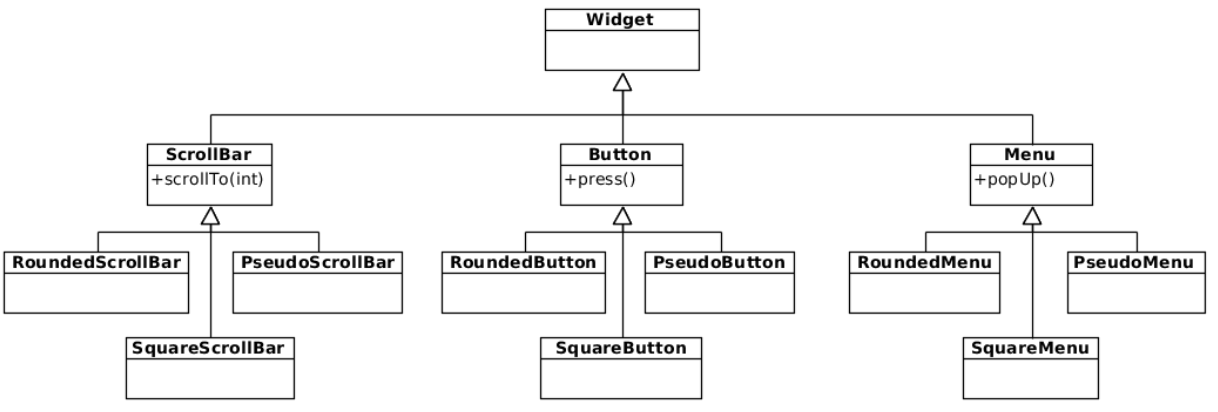
\includegraphics[width=0.95\textwidth]{widgets.png}
        \end{center}
    \end{frame}

    \begin{frame}{Создание виджетов}
        \mintinline{c++}|ScrollBar* bar = new RoundedScrollBar;|
        
        \vspace{2mm}
        
        vs
        
        \vspace{2mm}
        
        \mintinline{c++}|ScrollBar* bar = guiFactory->createScrollBar();|
    \end{frame}

    \begin{frame}{Фабрика виджетов}
        \begin{center}
            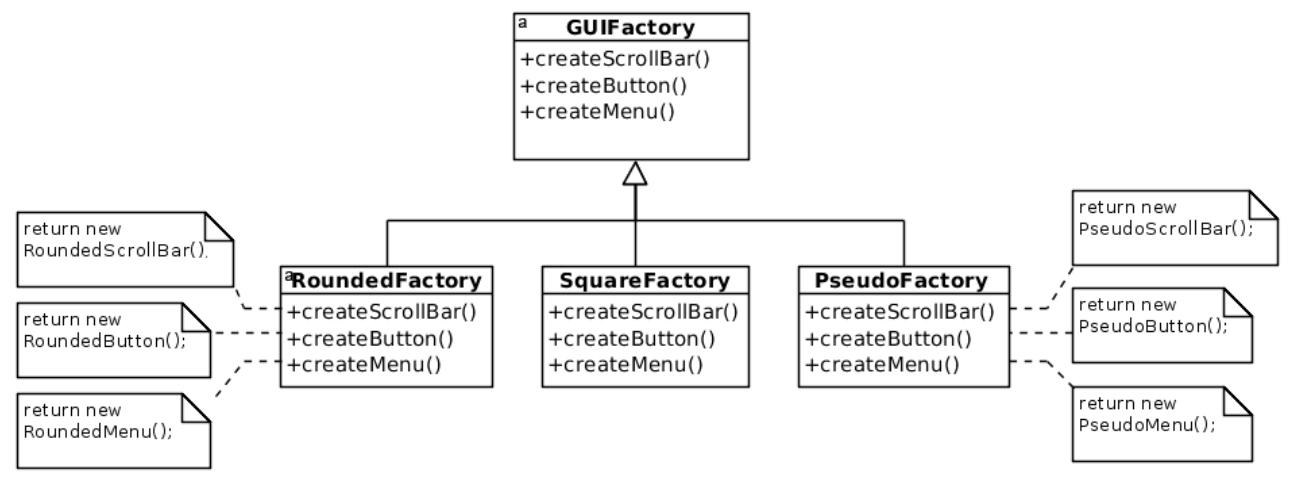
\includegraphics[width=0.95\textwidth]{widgetFactory.png}
        \end{center}
    \end{frame}

    \begin{frame}{Паттерн \enquote{Абстрактная фабрика}}
        \framesubtitle{Abstract Factory}
        \begin{columns}
            \begin{column}{0.4\textwidth}
                \begin{outline}
                    \1 Изолирует конкретные классы
                    \1 Упрощает замену семейств продуктов
                    \1 Гарантирует сочетаемость продуктов
                    \1 Поддержать новый вид продуктов непросто
                \end{outline}
            \end{column}
            \begin{column}{0.6\textwidth}
                \begin{center}
                    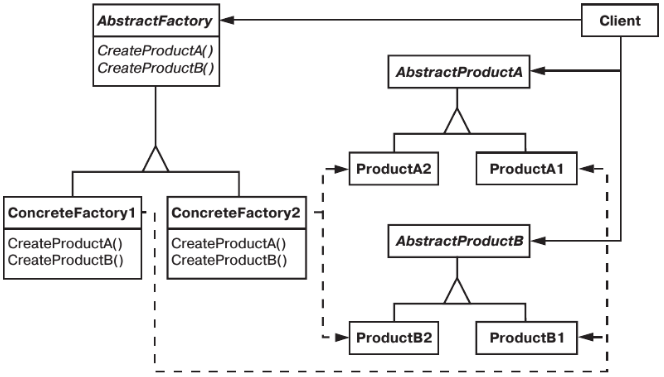
\includegraphics[width=0.95\textwidth]{abstractFactory.png}
                \end{center}
            \end{column}
        \end{columns}
    \end{frame}

    \begin{frame}{\enquote{Абстрактная фабрика}, применимость}
        \begin{outline}
            \1 Система не должна зависеть от того, как создаются, компонуются и представляются входящие в неё объекты
            \1 Система должна конфигурироваться одним из семейств составляющих её объектов
            \1 Взаимосвязанные объекты должны использоваться вместе
            \1 Хотите предоставить библиотеку объектов, раскрывая только их интерфейсы, но не реализацию
        \end{outline}
    \end{frame}

    \begin{frame}{\enquote{Абстрактная фабрика}, детали реализации}
        \begin{columns}
            \begin{column}{0.5\textwidth}
                \begin{outline}
                    \1 Хорошо комбинируются с паттерном \enquote{Одиночка}
                    \1 Если семейств продуктов много, то фабрика может инициализироваться \textit{прототипами}, тогда не надо создавать сотню подклассов
                \end{outline}
            \end{column}
            \begin{column}{0.5\textwidth}
                \begin{center}
                    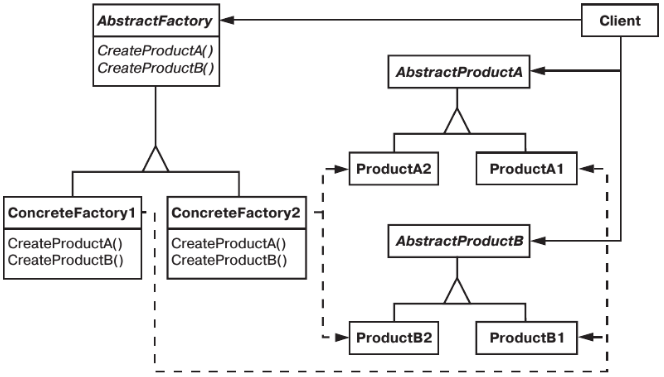
\includegraphics[width=\textwidth]{abstractFactory.png}
                \end{center}
            \end{column}
        \end{columns}
        \begin{outline}
            \1 Прототип на самом деле может быть классом (например, Class в Java)
            \1 Если виды объектов часто меняются, может помочь параметризация метода создания
                \2 Может пострадать типобезопасность
        \end{outline}
    \end{frame}

    \section{Паттерн \enquote{Прототип}}

    \begin{frame}{\enquote{Прототип}, мотивация}
        \begin{center}
            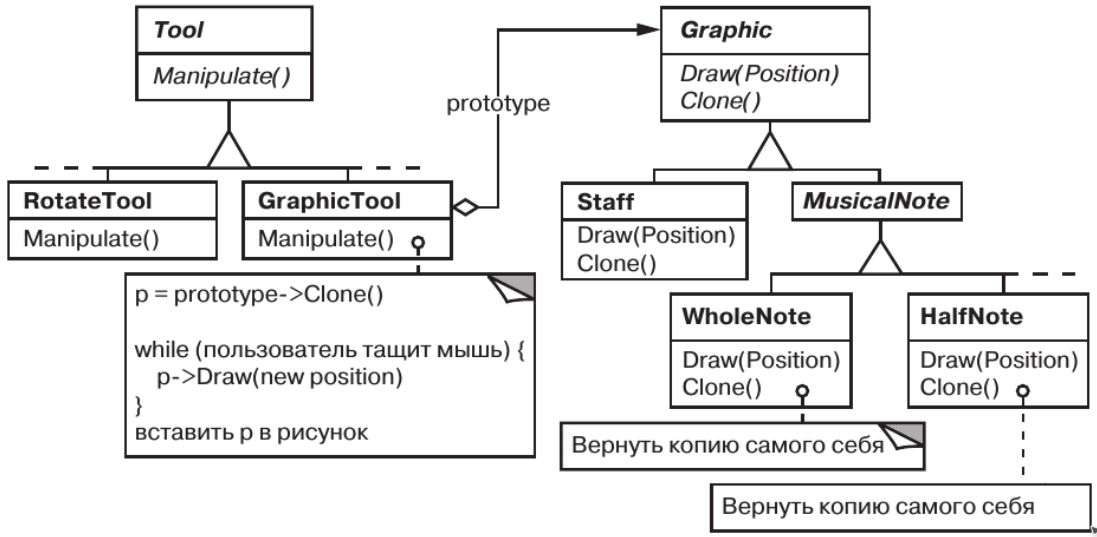
\includegraphics[width=0.9\textwidth]{musicalEditor.png}
        \end{center}
    \end{frame}

    \begin{frame}{Паттерн \enquote{Прототип}}
        \framesubtitle{Prototype}
        \begin{center}
            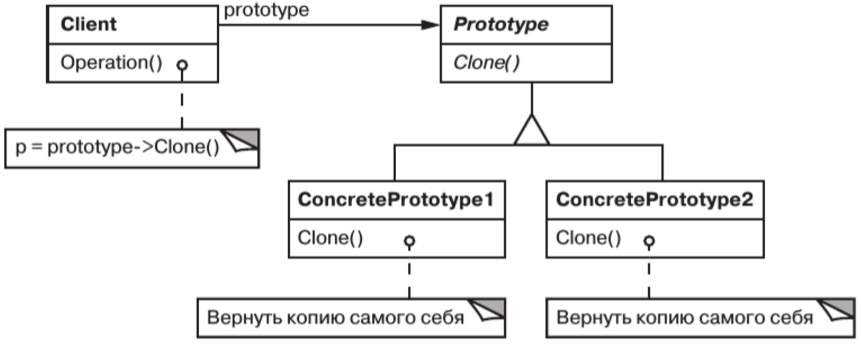
\includegraphics[width=0.85\textwidth]{prototype.png}
        \end{center}
    \end{frame}
    
    \begin{frame}{\enquote{Прототип}, детали реализации}
        \begin{outline}
            \1 Реестр прототипов, обычно ассоциативное хранилище
            \1 Операция Clone
                \2 Глубокое и мелкое копирование
                \2 В случае, если могут быть круговые ссылки
                \2 Сериализовать/десериализовать объект (но помнить про идентичность)
            \1 Инициализация клона
                \2 Передавать параметры в Clone --- плохая идея
        \end{outline}
    \end{frame}

    \section{Паттерн \enquote{Строитель}}

    \begin{frame}{\enquote{Строитель}, мотивация}
        \framesubtitle{Конвертер текста}
        \begin{center}
            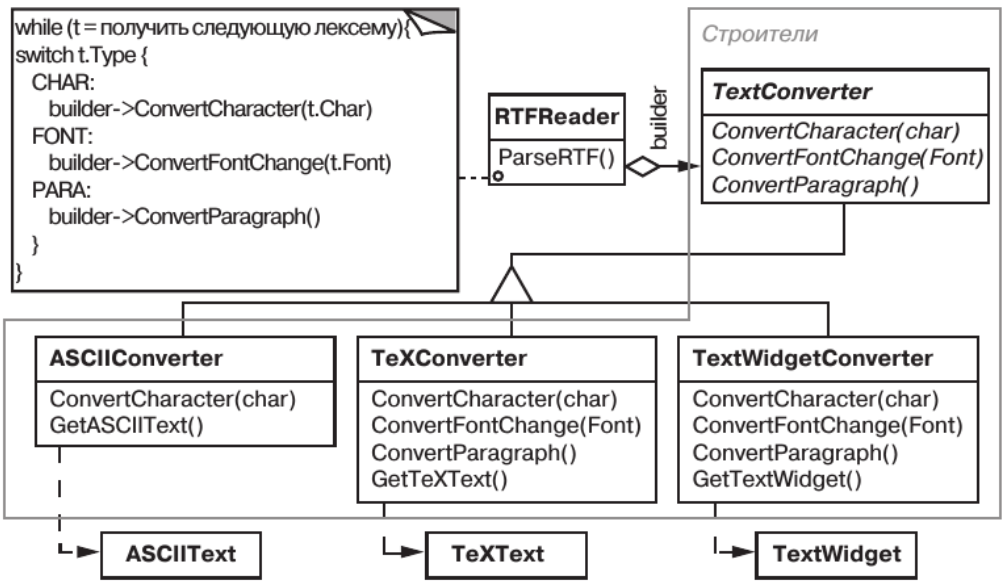
\includegraphics[width=0.8\textwidth]{textConverter.png}
        \end{center}
    \end{frame}

    \begin{frame}{Паттерн \enquote{Строитель}}
        \framesubtitle{Builder}
        \begin{center}
            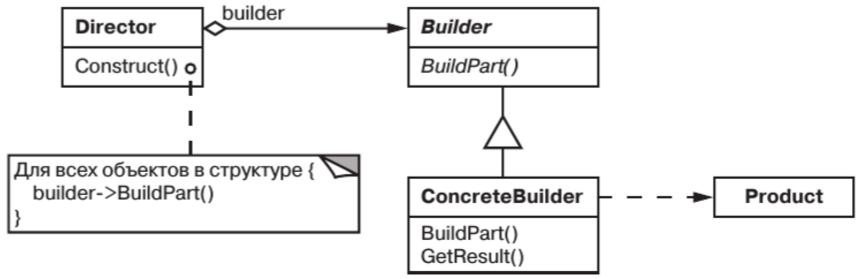
\includegraphics[width=0.85\textwidth]{builder.png}
        \end{center}
    \end{frame}
    
    \begin{frame}{\enquote{Строитель} (Builder), детали реализации}
        \begin{center}
            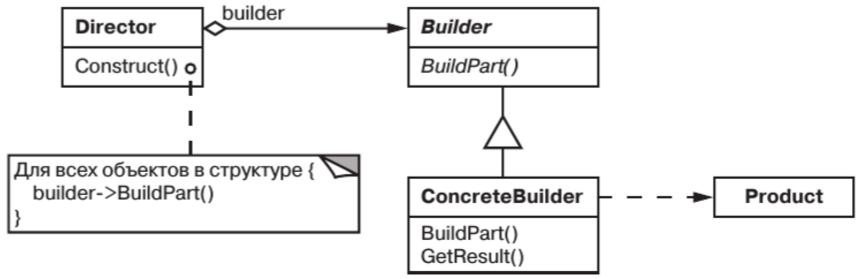
\includegraphics[width=0.7\textwidth]{builder.png}
        \end{center}
        \begin{outline}
            \1 Абстрактные и конкретные строители
                \2 Достаточно общий интерфейс
            \1 Общий интерфейс для продуктов не требуется
                \2 Клиент конфигурирует распорядителя конкретным строителем, он же и забирает результат
            \1 Пустые методы по умолчанию
        \end{outline}
    \end{frame}

    \begin{frame}[fragile]{\enquote{Строитель}, примеры}
        \begin{outline}
            \1 StringBuilder
            \1 Guava, подсистема работы с графами
            \begin{minted}{java}
MutableNetwork<Webpage, Link> webSnapshot = 
        NetworkBuilder.directed()
    .allowsParallelEdges(true)
    .nodeOrder(ElementOrder.natural())
    .expectedNodeCount(100000)
    .expectedEdgeCount(1000000)
    .build();
            \end{minted}
        \end{outline}
    \end{frame}

    \section{Задание}

    \begin{frame}{Задание на дом}
        Уточнить модель компьютерной игры Roguelike:

        \begin{outline}[enumerate]
            \1 Используя шаблон \enquote{Строитель} для инициализации карты
            \1 Используя шаблон \enquote{Абстрактная фабрика} для создания мобов и предметов на карте
            \1 Используя шаблон \enquote{Прототип} для поддержки клонирования персонажей и предметов
        \end{outline}

        Выложить модифицированные диаграммы классов в HwProj
    \end{frame}

\end{document}